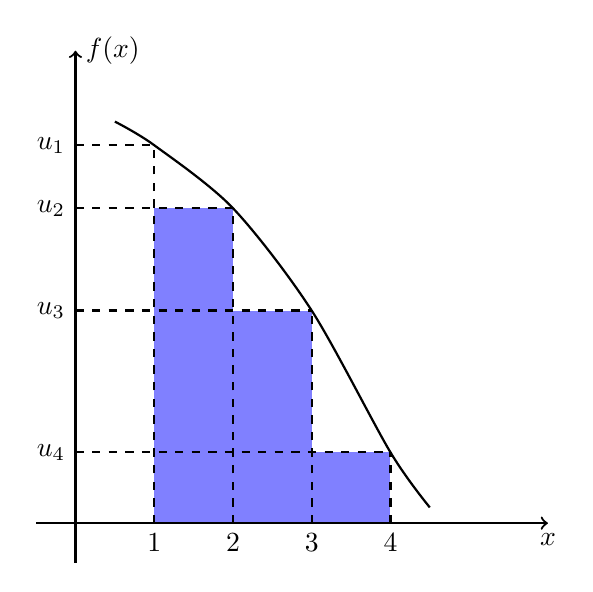
\begin{tikzpicture}
  
  \foreach \y [count = \x from 1] in {4, 2.7, 0.9} {
    \draw[fill = blue!50, draw = none]
      (\x, 0) rectangle ++(1, \y);
  }

  \draw[->, thick] (-0.5, 0) -- (6, 0)
    node[below] {\(x\)};
  \draw[->, thick] (0, -0.5) -- (0, 6)
    node[right] {\(f(x)\)};

  \foreach \y [count = \x from 1] in {4.8, 4, 2.7, 0.9} {
    \draw[dashed, thick] (0, \y) -- (\x, \y)
      node[pos = 0, left] {\(u_{\x}\)};
    \draw[dashed, thick] (\x, 0) -- (\x, \y)
      node[pos = 0, below] {\(\x\)};
  }

  \draw[thick] plot[smooth] coordinates {
    (0.5, 5.1) (1, 4.8) (2, 4) (3, 2.7) (4, 0.9) (4.5, 0.2)
  };

\end{tikzpicture}